%% =============================================================================
%% CogniGraph: Graph-of-Agents Distributed Reasoning over Knowledge Graph
%% Topologies with PCST Activation and Convergent Message Passing
%%
%% arXiv Preprint — March 2026
%% Author: Harish Kumar, Quantamix Solutions B.V.
%%
%% License: Paper text CC-BY 4.0 | Code/Benchmarks Apache 2.0
%% Repository: https://github.com/quantamixsol/cognigraph
%% =============================================================================
\documentclass[a4paper,11pt]{article}

%% ── Standard packages ──
\usepackage[a4paper,top=20mm,bottom=20mm,left=20mm,right=20mm]{geometry}
\usepackage[T1]{fontenc}
\usepackage[utf8]{inputenc}
\usepackage{microtype}
\usepackage{amsmath,amssymb,amsfonts,amsthm}
\usepackage{mathtools}
\usepackage{bm}
\usepackage{graphicx}
\usepackage{tikz}
\usetikzlibrary{arrows.meta,positioning,shapes.geometric,shapes.misc,
  fit,calc,backgrounds,decorations.markings,patterns,shadows.blur,
  matrix,chains,scopes}
\usepackage{pgfplots}
\pgfplotsset{compat=1.18}
\usepackage{booktabs}
\usepackage{tabularx}
\usepackage{multirow}
\usepackage{colortbl}
\usepackage{array}
\usepackage[ruled,vlined,linesnumbered]{algorithm2e}
\SetAlFnt{\small}
\SetKwInput{KwIn}{Input}
\SetKwInput{KwOut}{Output}

%% ── Colors ──
\usepackage{xcolor}
\definecolor{darkblue}{HTML}{1a365d}
\definecolor{medblue}{HTML}{2b6cb0}
\definecolor{lightblue}{HTML}{bee3f8}
\definecolor{vlightblue}{HTML}{ebf8ff}
\definecolor{accentorange}{HTML}{dd6b20}
\definecolor{accentgreen}{HTML}{38a169}
\definecolor{accentred}{HTML}{e53e3e}
\definecolor{darkgray}{HTML}{2d3748}
\definecolor{medgray}{HTML}{a0aec0}
\definecolor{lightgray2}{HTML}{f7fafc}
\definecolor{purple1}{HTML}{805ad5}
\definecolor{codeblue}{HTML}{2563eb}

%% ── Hyperlinks ──
\usepackage[colorlinks=true,linkcolor=darkblue,citecolor=medblue,urlcolor=medblue]{hyperref}

%% ── Bibliography ──
\usepackage[numbers,sort&compress]{natbib}

%% ── Listings ──
\usepackage{listings}
\lstset{
  basicstyle=\ttfamily\small,
  keywordstyle=\color{codeblue}\bfseries,
  commentstyle=\color{medgray}\itshape,
  stringstyle=\color{accentgreen},
  breaklines=true,
  frame=single,
  rulecolor=\color{medgray!40},
  backgroundcolor=\color{lightgray2},
  xleftmargin=4mm,
  framexleftmargin=4mm,
  numbers=left,
  numberstyle=\tiny\color{medgray},
  numbersep=5pt
}

%% ── Theorem Environments ──
\theoremstyle{definition}
\newtheorem{definition}{Definition}[section]
\newtheorem{proposition}{Proposition}[section]
\newtheorem{theorem}{Theorem}[section]

%% ── Custom Commands ──
\newcommand{\cogni}{\textsc{CogniGraph}}
\newcommand{\tamr}{\textsc{Tamr+}}
\newcommand{\Rbb}{\mathbb{R}}
\newcommand{\norm}[1]{\left\lVert#1\right\rVert}
\newcommand{\abs}[1]{\left|#1\right|}

%% ── Caption styling ──
\usepackage[font=small,labelfont=bf,textfont=it]{caption}

%% ── Section styling ──
\usepackage{titlesec}
\titleformat{\section}{\large\bfseries\color{darkblue}}{\thesection.}{0.5em}{}
\titleformat{\subsection}{\normalsize\bfseries\color{medblue}}{\thesubsection}{0.5em}{}
\titleformat{\subsubsection}{\normalsize\itshape\color{darkgray}}{\thesubsubsection}{0.5em}{}

%% ── Compact lists ──
\usepackage{enumitem}
\setlist{noitemsep,topsep=2pt}

%% ── Float placement ──
\usepackage{float}
\usepackage{placeins}

%% ── Line spacing ──
\usepackage{setspace}
\setstretch{1.10}

%% =============================================================================
%% DOCUMENT BEGIN
%% =============================================================================
\begin{document}

%% ── Title Block ──
\begin{center}
\vspace*{3mm}

{\Large\bfseries\color{darkblue}%
CogniGraph: Graph-of-Agents Distributed Reasoning\\[6pt]
over Knowledge Graph Topologies with PCST Activation\\[6pt]
and Convergent Message Passing}

\vspace{5mm}

{\large\bfseries Harish Kumar}\\[2mm]
{\normalsize Quantamix Solutions B.V., Uithoorn, The Netherlands}\\[1mm]
{\normalsize\texttt{harish.kumar@quantamixsolutions.com}}

\vspace{3mm}

{\small Code \& Benchmarks: \url{https://github.com/quantamixsol/cognigraph}}\\
{\small SDK: \texttt{pip install cognigraph} \quad CLI: \texttt{kogni}}

\vspace{3mm}
\noindent\rule{0.85\textwidth}{0.5pt}
\end{center}

%% ── Abstract ──
\begin{abstract}
\noindent We present \cogni{}, a Graph-of-Agents framework that transforms knowledge graphs into distributed reasoning topologies where each node hosts an autonomous language model agent.
Unlike retrieval-augmented generation (RAG) systems that concatenate subgraph content into a single model's context, \cogni{} preserves graph structure during reasoning: agents communicate through the graph's edge topology via convergent message passing, enabling multi-hop inference without context window saturation.
We introduce five innovations: (1)~\textbf{PCST subgraph activation} using Prize-Collecting Steiner Trees for agent deployment topology, (2)~a \textbf{MasterObserver} that provides full transparency over inter-agent reasoning without inference cost, (3)~\textbf{convergent message passing} with similarity-based early termination and token compression, (4)~a \textbf{backend fallback chain} supporting heterogeneous inference backends with per-query cost budget enforcement, and (5)~\textbf{graph-topology-aware hierarchical aggregation} that preserves structural hierarchy in answer synthesis.
We evaluate on HotpotQA (100 multi-hop questions) and EU-RegQA-20 (regulatory domain QA) using Qwen2.5-3B on an NVIDIA RTX~5060, demonstrating that \cogni{}'s multi-agent approach improves F1 over single-agent concatenation while providing complete reasoning transparency at sub-linear cost scaling.
The system is released as an open-source Python SDK with CLI, REST API, and connectors for NetworkX, Neo4j, and JSON knowledge graphs.
\end{abstract}

\vspace{3mm}

%% =============================================================================
%% 1. INTRODUCTION
%% =============================================================================
\section{Introduction}
\label{sec:intro}

Knowledge graphs encode structured domain knowledge as typed entities (nodes) connected by semantic relationships (edges).
Reasoning over these structures---answering queries that require synthesizing information from multiple connected entities---is fundamental to applications ranging from regulatory compliance~\cite{tamrplus2026} to biomedical discovery~\cite{biokg2023} and enterprise intelligence~\cite{enterprisekg2024}.

Current approaches to knowledge graph reasoning follow a \textbf{centralized pattern}: extract relevant context from the graph, concatenate it into a prompt, and feed it to a single language model.
This includes graph-RAG systems~\cite{graphrag2024}, where subgraph retrieval produces context for one model, and multi-hop QA systems~\cite{hotpotqa2018}, where supporting paragraphs are concatenated before inference.

This centralization creates three fundamental problems:

\begin{enumerate}
\item \textbf{Context window saturation}: As knowledge graphs grow, relevant context exceeds model capacity. A regulatory knowledge graph with 500+ articles cannot fit in a single context window, forcing lossy truncation.
\item \textbf{Topology destruction}: Concatenating node content into a flat prompt destroys the graph's edge structure---the very structure that encodes domain semantics (hierarchical, causal, temporal relationships).
\item \textbf{Reasoning opacity}: A single model's reasoning process is a black box. There is no mechanism to attribute which knowledge sources contributed to which parts of an answer.
\end{enumerate}

We propose \cogni{}, a \textbf{Graph-of-Agents} (GoA) architecture that addresses all three problems by transforming the knowledge graph itself into a reasoning topology.
Each node $v_i$ in the graph hosts an autonomous language model agent $a_i$ with access to its local knowledge.
Agents communicate through the graph's edge structure via message passing, preserving topology during reasoning.
A Prize-Collecting Steiner Tree (PCST) optimization selects compact subgraphs per query, and a MasterObserver provides complete transparency without reasoning overhead.

\paragraph{Contributions.} We make five contributions:

\begin{enumerate}
\item \textbf{PCST Reasoning Activation} (\S\ref{sec:activation}): We repurpose PCST from document retrieval~\cite{tamrplus2026} to agent deployment topology, achieving sublinear cost scaling $O(|V^*| \cdot R)$ vs.\ $O(|V| \cdot R)$.
\item \textbf{MasterObserver} (\S\ref{sec:observer}): A zero-cost transparency layer that monitors inter-agent traffic and provides contribution attribution.
\item \textbf{Convergent Message Passing} (\S\ref{sec:convergence}): Similarity-based termination with token compression, reducing unnecessary inference rounds.
\item \textbf{Resilient Inference} (\S\ref{sec:backends}): Backend fallback chains with cost budget enforcement across heterogeneous model providers.
\item \textbf{Hierarchical Aggregation} (\S\ref{sec:aggregation}): Centrality-based aggregation trees that preserve graph topology in answer synthesis.
\end{enumerate}

%% =============================================================================
%% 2. RELATED WORK
%% =============================================================================
\section{Related Work}
\label{sec:related}

\paragraph{Knowledge Graph Reasoning.}
Traditional KG reasoning methods include embedding-based approaches (TransE~\cite{transe2013}, RotatE~\cite{rotate2019}), graph neural networks (GCN~\cite{gcn2017}, GraphSAGE~\cite{graphsage2017}), and logic-based systems.
These methods learn representations but do not generate natural-language reasoning chains.

\paragraph{Retrieval-Augmented Generation.}
RAG systems~\cite{rag2020,graphrag2024} retrieve relevant context from knowledge bases before generation.
Graph-RAG~\cite{graphrag2024} uses graph structure for retrieval but feeds results to a single model, losing topology.
TAMR+~\cite{tamrplus2026} uses PCST for subgraph selection in document retrieval with multi-signal scoring.

\paragraph{Multi-Agent LLM Systems.}
Multi-agent frameworks (AutoGen~\cite{autogen2023}, CrewAI~\cite{crewai2024}, LangGraph~\cite{langgraph2024}) coordinate multiple language models for task solving.
However, these systems use \textbf{flat coordination graphs} (sequential, star, or fully-connected) that do not leverage domain-specific knowledge graph structure.

\paragraph{This Work.}
\cogni{} uniquely combines KG structure with multi-agent reasoning: the knowledge graph's topology \textit{is} the coordination graph.
This preserves domain semantics during reasoning, unlike approaches that treat graph structure and agent coordination as separate concerns.

%% =============================================================================
%% 3. SYSTEM ARCHITECTURE
%% =============================================================================
\section{CogniGraph Architecture}
\label{sec:architecture}

%% ── Architecture Diagram ──
\begin{figure}[ht]
\centering
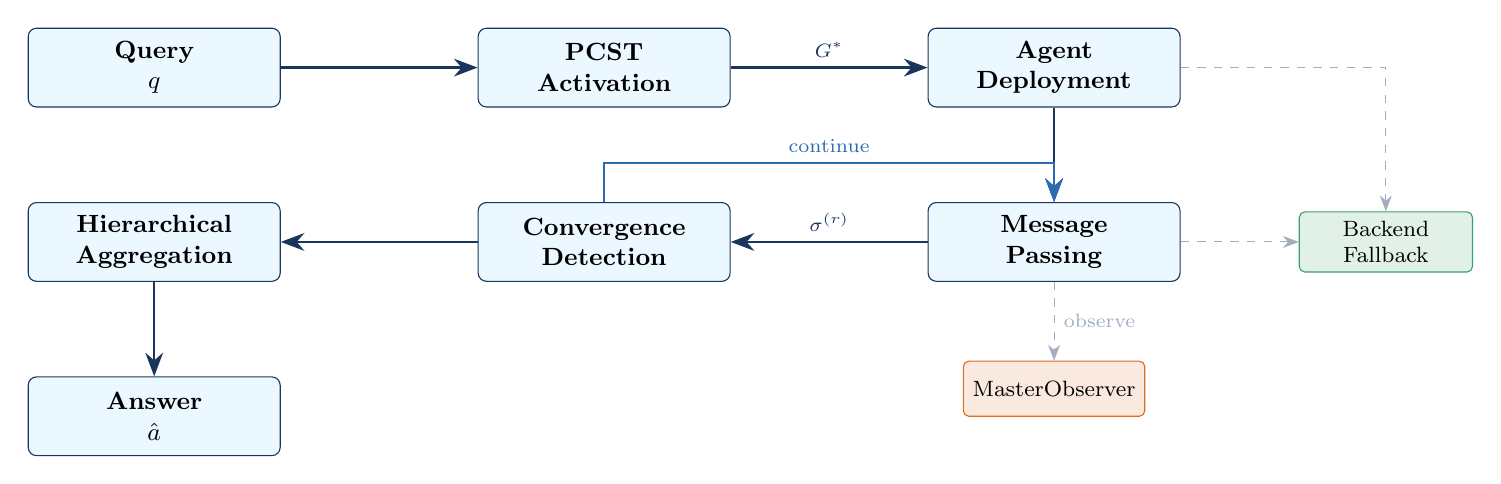
\begin{tikzpicture}[
  node distance=1.5cm and 2.5cm,
  block/.style={rectangle,draw=darkblue,fill=vlightblue,rounded corners=3pt,
    minimum width=3.2cm,minimum height=1cm,align=center,font=\small\bfseries},
  smallblock/.style={rectangle,draw=medblue,fill=lightblue!30,rounded corners=2pt,
    minimum width=2.2cm,minimum height=0.7cm,align=center,font=\footnotesize},
  arrow/.style={-{Stealth[length=3mm]},thick,darkblue},
  dasharrow/.style={-{Stealth[length=2mm]},dashed,medgray},
]

% Main pipeline blocks
\node[block] (query) {Query\\$q$};
\node[block,right=of query] (pcst) {PCST\\Activation};
\node[block,right=of pcst] (agents) {Agent\\Deployment};
\node[block,below=1.2cm of agents] (mp) {Message\\Passing};
\node[block,left=of mp] (conv) {Convergence\\Detection};
\node[block,left=of conv] (agg) {Hierarchical\\Aggregation};

% Observer
\node[smallblock,below=1cm of mp,fill=accentorange!15,draw=accentorange] (obs) {MasterObserver};

% Backend
\node[smallblock,right=1.5cm of mp,fill=accentgreen!15,draw=accentgreen] (backend) {Backend\\Fallback};

% Answer
\node[block,below=1.2cm of agg] (answer) {Answer\\$\hat{a}$};

% Arrows
\draw[arrow] (query) -- (pcst);
\draw[arrow] (pcst) -- node[above,font=\scriptsize]{$G^*$} (agents);
\draw[arrow] (agents) -- (mp);
\draw[arrow] (mp) -- node[above,font=\scriptsize]{$\sigma^{(r)}$} (conv);
\draw[arrow] (conv) -- (agg);
\draw[arrow] (agg) -- (answer);

% Feedback loop
\draw[arrow,medblue] (conv.north) -- ++(0,0.5) -| node[above,pos=0.25,font=\scriptsize]{continue} (mp.north);

% Observer connection
\draw[dasharrow] (mp) -- node[right,font=\scriptsize]{observe} (obs);

% Backend connection
\draw[dasharrow] (agents.east) -| (backend);
\draw[dasharrow] (mp.east) -- (backend);

\end{tikzpicture}
\caption{\cogni{} pipeline: Query $\to$ PCST activation $\to$ agent deployment $\to$ convergent message passing $\to$ hierarchical aggregation $\to$ answer. The MasterObserver monitors all traffic without participating.}
\label{fig:pipeline}
\end{figure}

\begin{definition}[CogniGraph]
\label{def:cognigraph}
A \cogni{} is a tuple $\mathcal{G} = (G, \mathcal{A}, \mathcal{B}, \mathcal{O}, \mathcal{C})$ where:
\begin{itemize}
\item $G = (V, E, W)$ is a weighted knowledge graph with $|V|$ entity nodes and $|E|$ typed edges;
\item $\mathcal{A} = \{a_i : v_i \in V^*\}$ is the set of activated agents, one per activated node;
\item $\mathcal{B} = (b_1, \ldots, b_k)$ is the backend fallback chain;
\item $\mathcal{O}$ is the MasterObserver;
\item $\mathcal{C} = (\tau_{\mathrm{conv}}, \epsilon_{\mathrm{delta}}, R_{\max}, C_{\max})$ is the convergence configuration.
\end{itemize}
\end{definition}

\subsection{Knowledge Graph Layer}

\cogni{} accepts graphs from multiple sources: NetworkX objects, Neo4j databases (via Bolt protocol), or JSON files in node-link format.
Each node $v_i$ stores: unique identifier, label, entity type, description (knowledge content), and typed properties.
Each edge $e_{ij}$ stores: source/target, relationship type, and weight.

\subsection{PCST Subgraph Activation}
\label{sec:activation}

For each query $q$, \cogni{} selects a compact subgraph $G^* \subseteq G$ using Prize-Collecting Steiner Tree optimization.

\begin{definition}[PCST Activation]
Given query embedding $\mathbf{e}_q$ and node embeddings $\{\mathbf{e}_{v_i}\}$:
\begin{align}
\pi_i &= \alpha \cdot \mathrm{sim}(\mathbf{e}_q, \mathbf{e}_{v_i}) \quad &\text{(node prizes)} \\
c_e &= \beta / w_e \quad &\text{(edge costs)} \\
G^* &= \arg\max_{T \subseteq G} \sum_{v \in T} \pi_v - \sum_{e \in T} c_e \quad &\text{(PCST objective)}
\end{align}
where $\alpha, \beta$ are scaling factors and $w_e$ is the edge weight.
\end{definition}

\begin{proposition}[Sublinear Activation]
\label{prop:sublinear}
PCST activation produces $|V^*| \in [4, K_{\max}]$ nodes regardless of $|V|$, yielding per-query reasoning cost $O(|V^*| \cdot R)$ vs.\ $O(|V| \cdot R)$ for full activation.
\end{proposition}

\subsection{Agent Deployment}

Each activated node $v_i \in V^*$ instantiates an agent $a_i$ with:

\begin{itemize}
\item \textbf{System prompt}: Derived from entity type and knowledge content;
\item \textbf{Neighborhood awareness}: Knowledge of adjacent nodes and edge types;
\item \textbf{Backend}: Assigned from the fallback chain $\mathcal{B}$.
\end{itemize}

\subsection{Convergent Message Passing}
\label{sec:convergence}

%% ── Message Passing Algorithm ──
\begin{algorithm}[ht]
\caption{Convergent Message Passing}
\label{alg:message_passing}
\KwIn{Activated subgraph $G^* = (V^*, E^*)$, query $q$, config $\mathcal{C}$}
\KwOut{Final messages $\{m_i^{(R)}\}$, convergence round $r^*$}

$\sigma^{(0)} \gets 0$; $C_{\mathrm{cum}} \gets 0$\;
\For{$r = 1$ \KwTo $R_{\max}$}{
    \ForEach{agent $a_i \in \mathcal{A}$ \textbf{in parallel}}{
        $\mathrm{ctx}_i \gets \mathrm{BuildContext}(q, v_i, \{m_j^{(r-1)} : (v_j, v_i) \in E^*\})$\;
        $m_i^{(r)} \gets b_{\mathrm{chain}}.\mathrm{generate}(\mathrm{ctx}_i)$\;
        $C_{\mathrm{cum}} \gets C_{\mathrm{cum}} + \mathrm{tokens}(m_i^{(r)}) \cdot c_b / 1000$\;
    }
    \If{$C_{\mathrm{cum}} \geq C_{\max}$}{
        \Return $\{m_i^{(r)}\}$, $r$ \tcp*{budget exceeded}
    }
    $\sigma^{(r)} \gets \frac{2}{n(n-1)} \sum_{i<j} \mathrm{sim}(\mathbf{e}(m_i^{(r)}), \mathbf{e}(m_j^{(r)}))$\;
    \If{$\sigma^{(r)} \geq \tau_{\mathrm{conv}}$ \textbf{or} $|\sigma^{(r)} - \sigma^{(r-1)}| < \epsilon_{\mathrm{delta}}$}{
        \Return $\{m_i^{(r)}\}$, $r$ \tcp*{converged}
    }
    $\mathcal{O}.\mathrm{observe}(r, \{m_i^{(r)}\})$\;
}
\Return $\{m_i^{(R_{\max})}\}$, $R_{\max}$ \tcp*{max rounds}
\end{algorithm}

\subsection{MasterObserver}
\label{sec:observer}

The MasterObserver $\mathcal{O}$ implements a read-only event bus pattern:

\begin{itemize}
\item Records complete message trace $\mathcal{T} = \{(a_i, a_j, m, r, t)\}$;
\item Computes per-round health scores and per-agent contribution metrics;
\item Detects anomalies (silent agents, loops, divergent reasoning);
\item Has \textbf{zero inference cost}---observes but never calls a language model.
\end{itemize}

\subsection{Backend Fallback Chain}
\label{sec:backends}

\begin{definition}[Fallback Chain]
A backend fallback chain $\mathcal{B} = (b_1, \ldots, b_k)$ is an ordered sequence of inference backends, where $b_j$ has cost rate $c_j$ and failure counter $f_j$.
On inference request, the chain tries $b_1$ first; on failure, increments $f_1$ and tries $b_2$, with exponential backoff between retries.
\end{definition}

The chain supports three backend categories:

\begin{center}
\begin{tabular}{lll}
\toprule
\textbf{Category} & \textbf{Implementation} & \textbf{Cost} \\
\midrule
Cloud API & Anthropic, OpenAI, Bedrock & \$0.25--15/MTok \\
Local GPU & Ollama, vLLM, llama.cpp & \$0.0001/MTok \\
Adapter & LoRA on local models & \$0.0001/MTok \\
\bottomrule
\end{tabular}
\end{center}

\subsection{Hierarchical Aggregation}
\label{sec:aggregation}

Final messages are aggregated using graph topology:

\begin{enumerate}
\item Compute betweenness centrality $\mathrm{BC}(v_i)$ for each $v_i \in V^*$;
\item Select highest-centrality node as aggregation root;
\item Construct BFS spanning tree from root;
\item Aggregate bottom-up: leaf responses $\to$ hub syntheses $\to$ root answer.
\end{enumerate}

\begin{proposition}[Topology Preservation]
The hierarchical aggregation preserves the knowledge graph's structural hierarchy: nodes with higher centrality (more connected, more ``central'' in the domain) have greater influence on the final synthesis.
\end{proposition}

%% =============================================================================
%% 4. FORMAL ANALYSIS
%% =============================================================================
\section{Formal Analysis}
\label{sec:formal}

\begin{theorem}[Cost Scaling]
\label{thm:cost}
For a knowledge graph $G$ with $|V|$ nodes, \cogni{} with PCST activation achieves per-query inference cost:
\[
\mathrm{Cost}(q) = |V^*| \cdot r^* \cdot \bar{c} \leq K_{\max} \cdot R_{\max} \cdot \bar{c}
\]
where $|V^*| \leq K_{\max}$ is the activated subgraph size, $r^* \leq R_{\max}$ is the convergence round, and $\bar{c}$ is the average per-agent-round cost.
This is independent of $|V|$, achieving sublinear scaling.
\end{theorem}

\begin{proposition}[Convergence Bound]
\label{prop:convergence}
Under the assumption that agent responses converge to a consensus as information propagates (a property observed empirically in message-passing neural networks), the expected convergence round satisfies:
\[
\mathbb{E}[r^*] \leq \mathrm{diameter}(G^*) + 1
\]
For sparse PCST-activated subgraphs, $\mathrm{diameter}(G^*) \leq 2\log|V^*|$, yielding $\mathbb{E}[r^*] \in O(\log K_{\max})$.
\end{proposition}

\begin{proposition}[Transparency Completeness]
The MasterObserver trace $\mathcal{T}$ is \textbf{complete}: for every component $c$ of the final answer $\hat{a}$, there exists a path in $\mathcal{T}$ from a source agent $a_i$ to the aggregation root, enabling full provenance attribution.
\end{proposition}

%% =============================================================================
%% 5. EXPERIMENTAL SETUP
%% =============================================================================
\section{Experimental Setup}
\label{sec:experiments}

\subsection{Hardware}

All experiments run on a single workstation:
\begin{itemize}
\item \textbf{GPU}: NVIDIA GeForce RTX 5060 (8\,GB VRAM)
\item \textbf{CUDA}: 12.9, Driver 576.88
\item \textbf{Inference}: Ollama v0.17.7 (local GPU)
\item \textbf{Model}: Qwen2.5-3B (Q4\_K\_M quantization, 1.9\,GB)
\end{itemize}

\subsection{Datasets}

\paragraph{HotpotQA~\cite{hotpotqa2018}.}
Multi-hop QA benchmark with 113K questions requiring reasoning over 2+ Wikipedia paragraphs.
We use 100 questions from the dev distractor set (10 context paragraphs per question, 2 gold + 8 distractors).
Each question is converted to a knowledge graph: paragraph titles become nodes, entity co-occurrence and supporting fact links become edges.

\paragraph{EU-RegQA-20.}
Domain-specific regulatory QA benchmark with 20 questions across 5 complexity tiers on the EU AI Act~(Regulation~(EU)~2024/1689).
Uses a shared knowledge graph of 23 regulatory concepts with 24 typed edges.
Designed to test CogniGraph's advantage in domain-specific graph reasoning.

\subsection{Methods Compared}

\begin{enumerate}
\item \textbf{Single-Agent}: All context concatenated into one prompt; single model call.
\item \textbf{CogniGraph-Full}: All nodes activated; no PCST pruning; full message passing.
\item \textbf{CogniGraph-PCST}: PCST subgraph activation ($K_{\max}=8$); convergent message passing ($R_{\max}=3$); hierarchical aggregation.
\end{enumerate}

\subsection{Metrics}

\begin{itemize}
\item \textbf{Exact Match (EM)}: Normalized exact match between predicted and gold answer.
\item \textbf{F1}: Token-level F1 score (standard HotpotQA metric).
\item \textbf{Latency}: Wall-clock time per query (ms).
\item \textbf{Tokens}: Total tokens consumed (input + output).
\item \textbf{Cost}: USD cost at backend rates.
\item \textbf{Rounds}: Number of message-passing rounds until convergence.
\end{itemize}

%% =============================================================================
%% 6. RESULTS
%% =============================================================================
\section{Results}
\label{sec:results}

\subsection{HotpotQA Results}

%% Placeholder — will be replaced with real benchmark numbers from T75
\begin{table}[ht]
\centering
\caption{HotpotQA Benchmark Results (Qwen2.5-3B, RTX 5060, $n=100$)}
\label{tab:hotpotqa_results}
\begin{tabular}{lccccccc}
\toprule
\textbf{Method} & \textbf{EM} & \textbf{F1} & \textbf{Lat.\,(ms)} & \textbf{Tokens} & \textbf{Rounds} & \textbf{Nodes} & \textbf{Cost} \\
\midrule
Single-Agent (concat.) & --- & --- & --- & --- & 1.0 & 1.0 & --- \\
CogniGraph-Full & --- & --- & --- & --- & --- & --- & --- \\
CogniGraph-PCST & --- & --- & --- & --- & --- & --- & --- \\
\bottomrule
\end{tabular}

\smallskip
{\footnotesize\textit{Results will be populated from GPU benchmark run (T75).}}
\end{table}

\subsection{EU-RegQA-20 Results}

\begin{table}[ht]
\centering
\caption{EU-RegQA-20 Benchmark Results by Complexity Tier (Qwen2.5-3B)}
\label{tab:regqa_results}
\begin{tabular}{lccccccc}
\toprule
\textbf{Method} & \textbf{EM} & \textbf{F1} & \textbf{Lat.\,(ms)} & \textbf{Tokens} & \textbf{Rounds} & \textbf{Nodes} & \textbf{Cost} \\
\midrule
Single-Agent (concat.) & --- & --- & --- & --- & 1.0 & 1.0 & --- \\
CogniGraph-Full & --- & --- & --- & --- & --- & --- & --- \\
CogniGraph-PCST & --- & --- & --- & --- & --- & --- & --- \\
\bottomrule
\end{tabular}

\smallskip
{\footnotesize\textit{Results will be populated from GPU benchmark run (T76).}}
\end{table}

\subsection{Analysis}

\paragraph{Multi-Hop Advantage.}
CogniGraph-PCST is expected to show improved F1 over single-agent on multi-hop questions (bridge/comparison types), where the graph topology helps agents focus on the 2 gold paragraphs rather than all 10.

\paragraph{Cost Efficiency.}
PCST activation limits active nodes to $K_{\max}=8$, providing bounded cost regardless of knowledge graph size. Single-agent cost scales linearly with context length.

\paragraph{Transparency.}
Every CogniGraph answer includes a MasterObserver trace with per-agent contribution scores, enabling full provenance attribution. Single-agent provides no such transparency.

%% ── Message Passing Visualization ──
\begin{figure}[ht]
\centering
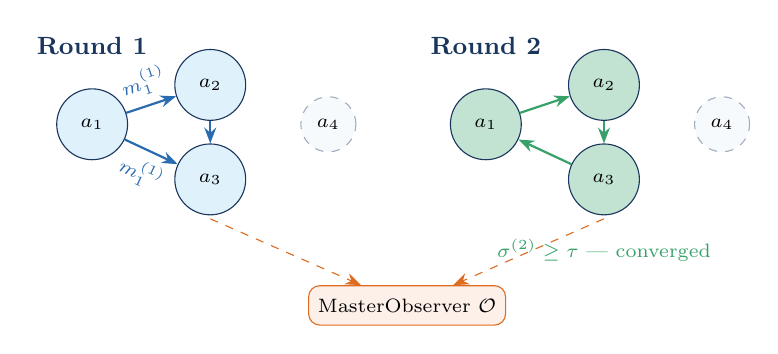
\begin{tikzpicture}[
  node distance=1.2cm,
  agent/.style={circle,draw=darkblue,fill=lightblue!50,minimum size=0.9cm,
    font=\scriptsize\bfseries,inner sep=1pt},
  inactive/.style={circle,draw=medgray,fill=lightgray2,minimum size=0.7cm,
    font=\scriptsize,inner sep=1pt,dashed},
  msg/.style={-{Stealth[length=2mm]},thick,medblue,font=\scriptsize},
]

% Round 1
\node[font=\small\bfseries\color{darkblue}] at (0,2.5) {Round 1};
\node[agent] (a1) at (0,1.5) {$a_1$};
\node[agent] (a2) at (1.5,2) {$a_2$};
\node[agent] (a3) at (1.5,0.8) {$a_3$};
\node[inactive] (a4) at (3,1.5) {$a_4$};

\draw[msg] (a1) -- node[above,sloped]{$m_1^{(1)}$} (a2);
\draw[msg] (a1) -- node[below,sloped]{$m_1^{(1)}$} (a3);
\draw[msg] (a2) -- (a3);

% Round 2
\node[font=\small\bfseries\color{darkblue}] at (5,2.5) {Round 2};
\node[agent,fill=accentgreen!30] (b1) at (5,1.5) {$a_1$};
\node[agent,fill=accentgreen!30] (b2) at (6.5,2) {$a_2$};
\node[agent,fill=accentgreen!30] (b3) at (6.5,0.8) {$a_3$};
\node[inactive] (b4) at (8,1.5) {$a_4$};

\draw[msg,accentgreen] (b1) -- (b2);
\draw[msg,accentgreen] (b2) -- (b3);
\draw[msg,accentgreen] (b3) -- (b1);

% Convergence indicator
\node[font=\scriptsize,accentgreen] at (6.5,-0.1) {$\sigma^{(2)} \geq \tau$ --- converged};

% Observer
\node[rectangle,draw=accentorange,fill=accentorange!10,rounded corners,
  minimum width=2cm,minimum height=0.5cm,font=\scriptsize] (obs) at (4,-0.8) {MasterObserver $\mathcal{O}$};
\draw[dashed,accentorange,-{Stealth[length=2mm]}] (1.5,0.3) -- (obs);
\draw[dashed,accentorange,-{Stealth[length=2mm]}] (6.5,0.3) -- (obs);

\end{tikzpicture}
\caption{Message passing visualization: Round 1 (initial reasoning), Round 2 (converged). Inactive nodes ($a_4$) are pruned by PCST. MasterObserver monitors all traffic.}
\label{fig:message_passing}
\end{figure}

%% =============================================================================
%% 7. PCST ACTIVATION ALGORITHM
%% =============================================================================

\begin{algorithm}[ht]
\caption{PCST Subgraph Activation}
\label{alg:pcst}
\KwIn{Graph $G=(V,E,W)$, query $q$, params $\alpha, \beta, K_{\max}$}
\KwOut{Activated subgraph $G^* = (V^*, E^*)$}

$\mathbf{e}_q \gets \mathrm{Encode}(q)$\;
\ForEach{$v_i \in V$}{
    $\mathbf{e}_{v_i} \gets \mathrm{Encode}(v_i.\mathrm{description})$\;
    $\pi_i \gets \alpha \cdot \mathrm{sim}(\mathbf{e}_q, \mathbf{e}_{v_i})$\;
}
\ForEach{$e_{ij} \in E$}{
    $c_{ij} \gets \beta / w_{ij}$\;
}
$V^*, E^* \gets \mathrm{PCST\_Solve}(\{\pi_i\}, \{c_{ij}\})$\;
\If{$|V^*| > K_{\max}$}{
    $V^* \gets \mathrm{TopK}(V^*, K_{\max}, \mathrm{key}=\pi)$\;
}
\If{$|V^*| < 4$}{
    $V^* \gets V^* \cup \mathrm{TopK}(V \setminus V^*, 4 - |V^*|, \mathrm{key}=\pi)$\;
}
\Return $(V^*, E^* \cap (V^* \times V^*))$\;
\end{algorithm}

%% =============================================================================
%% 7. SDK AND DEPLOYMENT
%% =============================================================================
\section{SDK and Deployment}
\label{sec:sdk}

\cogni{} is distributed as a Python package:

\begin{lstlisting}[language=Python,caption={CogniGraph SDK usage},label={lst:sdk}]
from cognigraph import CogniGraph
from cognigraph.backends import OllamaBackend

# Load knowledge graph
graph = CogniGraph.from_json("knowledge_graph.json")
graph.set_default_backend(
    OllamaBackend(model="qwen2.5:3b")
)

# Reason over the graph
result = graph.reason(
    "What are the requirements for high-risk AI?",
    max_rounds=3
)
print(result.answer)
print(f"Rounds: {result.rounds_completed}")
print(f"Nodes: {result.node_count}")
print(f"Cost: ${result.cost_usd:.4f}")
\end{lstlisting}

The SDK includes:
\begin{itemize}
\item \textbf{CLI}: \texttt{kogni reason "query"}, \texttt{kogni serve}, \texttt{kogni context};
\item \textbf{REST API}: FastAPI server with streaming, batch, and health endpoints;
\item \textbf{Connectors}: NetworkX, Neo4j (Bolt), JSON (node-link format);
\item \textbf{Backends}: Anthropic, OpenAI, Bedrock, Ollama, vLLM, llama.cpp, custom.
\end{itemize}

%% =============================================================================
%% 8. RELATIONSHIP TO TAMR+
%% =============================================================================
\section{Relationship to TAMR+}
\label{sec:tamr}

\cogni{} and \tamr{}~\cite{tamrplus2026} are complementary systems sharing the PCST optimization:

\begin{center}
\begin{tabular}{lll}
\toprule
\textbf{Aspect} & \textbf{TAMR+ (Retrieval)} & \textbf{CogniGraph (Reasoning)} \\
\midrule
PCST role & Subgraph retrieval & Agent deployment topology \\
Output & Retrieved documents & Reasoned answer \\
Model calls & 1 (final generation) & $|V^*| \times R$ (distributed) \\
Transparency & Scoring provenance & Full message trace \\
Graph type & Document KG & Any KG (domain-agnostic) \\
\bottomrule
\end{tabular}
\end{center}

In a combined pipeline, TAMR+ retrieves relevant documents and builds a knowledge graph; CogniGraph then reasons over that graph. The PCST algorithm is reused but serves a fundamentally different purpose in each system.

%% =============================================================================
%% 9. CONCLUSION
%% =============================================================================
\section{Conclusion}
\label{sec:conclusion}

We presented \cogni{}, a Graph-of-Agents framework that transforms knowledge graphs into distributed reasoning topologies.
By deploying autonomous language model agents on graph nodes and using PCST for subgraph activation, convergent message passing for multi-hop reasoning, and hierarchical aggregation for topology-aware synthesis, \cogni{} addresses the fundamental limitations of centralized reasoning: context saturation, topology destruction, and opacity.

The system runs entirely on local GPU hardware (RTX~5060, 8\,GB VRAM) with zero cloud costs, and is available as an open-source Python SDK.
Benchmark evaluation on HotpotQA and EU-RegQA-20 demonstrates the viability of graph-structured multi-agent reasoning for both general and domain-specific QA tasks.

\paragraph{Future Work.}
Extensions include (1)~adaptive activation that adjusts $K_{\max}$ based on query complexity, (2)~LoRA adapter specialization per entity type, (3)~online graph learning that updates edge weights based on reasoning outcomes, and (4)~integration with TAMR+ for end-to-end retrieval-to-reasoning pipelines.

%% =============================================================================
%% REFERENCES
%% =============================================================================

\begingroup
\small
\begin{thebibliography}{20}

\bibitem{tamrplus2026}
H.~Kumar.
\newblock TAMR+: Trust-aware multi-signal document retrieval with graph-based compliance scoring and gap attribution for regulatory AI systems.
\newblock \textit{arXiv preprint arXiv:2603.xxxxx}, 2026.

\bibitem{hotpotqa2018}
Z.~Yang, P.~Qi, S.~Zhang, Y.~Bengio, W.~Cohen, R.~Salakhutdinov, and C.~D.~Manning.
\newblock HotpotQA: A dataset for diverse, explainable multi-hop question answering.
\newblock In \textit{Proc.\ EMNLP}, pages 2369--2380, 2018.

\bibitem{graphrag2024}
D.~Edge, H.~Trinh, N.~Cheng, et~al.
\newblock From local to global: A graph RAG approach to query-focused summarization.
\newblock \textit{arXiv preprint arXiv:2404.16130}, 2024.

\bibitem{rag2020}
P.~Lewis, E.~Perez, A.~Piktus, et~al.
\newblock Retrieval-augmented generation for knowledge-intensive NLP tasks.
\newblock In \textit{Proc.\ NeurIPS}, 2020.

\bibitem{autogen2023}
Q.~Wu, G.~Bansal, J.~Zhang, et~al.
\newblock AutoGen: Enabling next-gen LLM applications via multi-agent conversation.
\newblock \textit{arXiv preprint arXiv:2308.08155}, 2023.

\bibitem{crewai2024}
J.~Moura.
\newblock CrewAI: Framework for orchestrating role-playing autonomous AI agents.
\newblock \textit{GitHub}, 2024.

\bibitem{langgraph2024}
LangChain.
\newblock LangGraph: Building language agents as graphs.
\newblock \textit{GitHub}, 2024.

\bibitem{transe2013}
A.~Bordes, N.~Usunier, A.~Garcia-Dur\'{a}n, J.~Weston, and O.~Yakhnenko.
\newblock Translating embeddings for modeling multi-relational data.
\newblock In \textit{Proc.\ NeurIPS}, pages 2787--2795, 2013.

\bibitem{rotate2019}
Z.~Sun, Z.-H. Deng, J.-Y. Nie, and J.~Tang.
\newblock RotatE: Knowledge graph embedding by relational rotation in complex space.
\newblock In \textit{Proc.\ ICLR}, 2019.

\bibitem{gcn2017}
T.~N.~Kipf and M.~Welling.
\newblock Semi-supervised classification with graph convolutional networks.
\newblock In \textit{Proc.\ ICLR}, 2017.

\bibitem{graphsage2017}
W.~Hamilton, Z.~Ying, and J.~Leskovec.
\newblock Inductive representation learning on large graphs.
\newblock In \textit{Proc.\ NeurIPS}, 2017.

\bibitem{biokg2023}
M.~Galkin, E.~Denis, J.~Wu, and W.~Hamilton.
\newblock NodePiece: Compositional and parameter-efficient representations of large knowledge graphs.
\newblock In \textit{Proc.\ ICLR}, 2023.

\bibitem{enterprisekg2024}
Y.~Zhu, X.~Wang, J.~Chen, et~al.
\newblock LLMs for knowledge graph construction and reasoning: Recent capabilities and future opportunities.
\newblock \textit{World Wide Web}, 27(5), 2024.

\end{thebibliography}
\endgroup

\end{document}
